\chapter{Methods}

\section{The data}
PLease tell where is the data come from, a little brief of company can be put here.

\section{Method 1}
Definition, steps, algoritm or equation of method 1 and how to apply into your data
\section{Method 2}
Definition, steps, algoritm or equation of method 2 and how to apply into your data

\section{Yusniar Nur Syarif Sidiq/1164089}
\begin{enumerate}

\item Random Forest merupakan algoritma yang digunakan terhadapap klasifikasi data dalam jumlah yang besar. Klasifikasi pada random forest dilakukan dengan penggabungan dicision tree dengan melakuakn training terhadap sempel data yang dimiliki. Semakin banyak dicision tree maka data yang di dapat akan semakin akurat. Untuk gambar Random Forest dapat dilihat pada figure \ref{YNRF}

	\begin{figure}[ht]
	\centerline{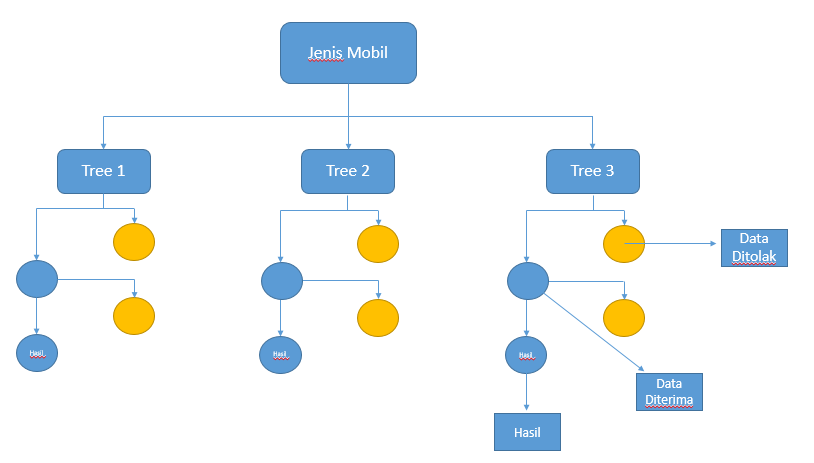
\includegraphics[width=1\textwidth]{figures/YN/RF.PNG}}
	\caption{Random Forest.}
	\label{YNRF}
	\end{figure}

\item Pertama download dataset terlebih dahulu lalu buka dengan menggunakan software spyder guna melihat isi dari dataset tersebut. Data tersebut memiliki extensi file bernama .txt dan didalamnya terdapat class dari field. Misalnya saja pada data jenis burung memiliki file index dan angka, dimana index berisi angka yang memiliki makna berupa jenis burung atau bahkan nama burung sedangkan field memiliki isi nilai berupa 0 dan 1 yang dimana sifatnya boolean atau Ya dan Tidak. Hal ini dikarenakan komputer hanya dapat membaca bilangan biner maka dari itu field yang di isikan berupa angka. Artinya angka 0 berarti tidak dan angka 1 berarti Ya.

\item Cross Validation adalah sebuah teknik validasi model yang digunakan untuk menilai bagaimana hasil analisis statistik akan digeneralisasi ke kumpulan data independen. Cross validation digunakan dengan tujuan prediksi, dan bila kita ingin memperkirakan seberapa akurat model model prediksi yang dilakukan dalam sebuah praktek. Tujuan dari cross validation yaitu untuk mendefinisikan dataset guna menguju dalam fase pelatihan untuk membatasi masalah seperti overfitting dan underfitting serta mendapatkan wawasan tentang bagaimana model akan digeneralisasikan ke set data independen.

\item Dimana Score 44 \% diperoleh dari hasil pengelohan dataset jenis burung. Dimana akan dilakukan proses pembagian data testing dan data training lalu diproses dan menghasilkan score sebanyak 44 \% dimana menjelaskan bahwa score tersebut digunakan sebagai pembanding dalam tingkat keakuratannya. Pada dicision tree akan memperoleh data lebih kecil yaitu sebanyak 27 \% hal ini dikarenakan data yang diolah menggunakan dicision tree dibagi menjadi beberapa tree dan lalu disimpulkan untuk mendapatkan data yang akurat. Pada SVM akan memperoleh score sebanyak 29 \% hal ini dikarenakan data yang dimiliki masih bernilai netral sehingga tingkat keakuratannya masih belum jelas.

\item Untuk membaca confusion matriks dapat menggunakan source code sebagai berikut,
	\begin{verbatim}
		import numpy as np
		np.set_printoptions(precision=2)
		plt.figure(figsize=(60,60), dpi=300)
		plot_confusion_matrix(cm, classes=birds, normalize=True)
		plt.show()
	\end{verbatim}

Dimana numpy akan mengurus semua data yang berhubungan dengan matrix. Pada source code tersebut digunakan dalam melakukan read pada dataset burung dengan menggunakan metode confusion matrix. Dalam confusion matrix memiliki 4 istilah yaitu True Positive yang merupakan data posotif yang terditeksi benar, True Negatif yang merupakan data negatif akan tetapi terditeksi benar, False Positif merupakan data negatif namun terditeksi sebagai data positif, False Negatif merupakan data posotif namun terditeksi sebagai data negatif. Adapun contoh hasil read dataset menggunakan confusion matrix dapat dilihat pada figure \ref{YNCM}
	
	\begin{figure}[ht]
	\centerline{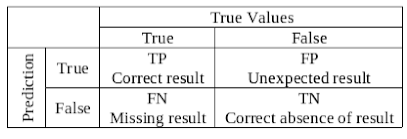
\includegraphics[width=1\textwidth]{figures/YN/YNCM.PNG}}
	\caption{Confusion Matrix.}
	\label{YNCM}
	\end{figure}

\item Voting merupakan proses pemilihan dari tree yang dimana akan dimunculkan hasilnya dan disimpulkan menjadi informasi yang pasti. Untuk kebih jelasnya saya akan memberikan sebuah contoh bagaimana voting beerja.
	
	\begin{figure}[ht]
	\centerline{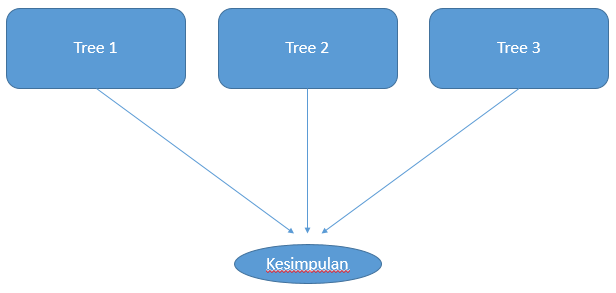
\includegraphics[width=1\textwidth]{figures/YN/YNVoting.PNG}}
	\caption{Voting.}
	\label{YNV}
	\end{figure}

Dimana ditunjukkan pada figure \ref{YNV} terdapat 3 tree. Dalam tree tersebut akan dilakukan proses voting. Saya akan memberikan contoh kasus, dimana akan diadakan voting untuk menentukan sebuah mobil. Dalam tree akan diberikan sejumlah data misalnya saja data tersebut berupa gambar, yang dimana data tersebut akan dipilih dengan cara voting. Hasil voting akhir dari setiap tree menunjukkan mobil jazz, yang berarti kesimpulan dari data yang telah diberikan menyatakan gambar tersebut adalah mobil jazz. Bagaimana apabila terjadi perbedaan data misalnya saja pada tree 1 dan 2 menunyatakan mobil jazz sedangkan pada tree 3 menyatakan mobil yaris, maka kesimpulan yang di ambil adalah mobil jazz dikarenakan hasil voting terbanyak adalah mobil jazz.

\end{enumerate}


\section{Imron Sumadireja/1164076}
\subsection{Teori}
\begin{enumerate}
\item Random Forest Beserta Ilustrasinya \par
Random Forest adalah salah satu algoritma yang digunakan pada klasifikasi data dalam jumlah yang besar. Klasifikasi random forest ini dilakukan melalui penggabungan decision tree dengan melakukan training pada sampel data yang dimiliki atau biasa disebut dengan supervised learning. Semakin banyak menggunakan decision tree maka akan mempengaruhi akurasi yang didapatkan menjadi lebih baik. Setiap decision tree memiliki atribut yang berbeda, serta decision tree tersebut spesifik terhadap atributnya yang merupakan bagian kecil dari keseluruhan atribut pada data set. Contoh sederhananya bisa dilihat pada gambar berikut \ref{R1}
		\begin{figure}[ht]
		\centerline{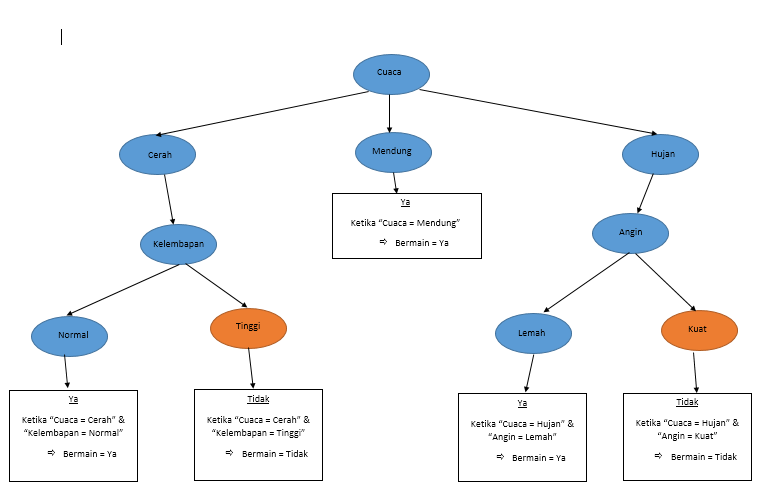
\includegraphics[width=1\textwidth]{figures/im/R1.png}}
		\caption{Random Forest.}
		\label{R1}
		\end{figure}

\item Membaca Dataset, Makna Setiap File Serta Field Masing-Masing File\par
Pertama download terlebih dahulu datasetnya kemudian buka menggunakan spyder untuk mengetahui isi dari dataset tersebut. Untuk menjalankan code tersebut tinggal blok bagian yang akan di jalankan. Dataset tersebut di dalamnya terdapat class dari field atau data. Sebagai contoh pada data burung terdapat field index dan angka, untuk index biasanya berupa angka, angka tersebut memiliki makna sebagai pengganti nama atau jenis burung. Sedangkan field berisi nilai 0 dan 1 maknanya untuk memberikan penilaian ya atau tidak pada setiap suatu data namun pada kasus ini field di ganti dari ya atau tidak menjadi 0 dan 1 karena komputer kesulitan membaca ya atau tidak dan hanya bisa membaca dengan 0 dan 1 saja.

\item Cross Validation \par
Cross validation adalah metode statistik yang dapat digunakan untuk mengevaluasi kinerja model atau algoritma dengan data dipisahkan menjadi dua subset yaitu data testing dan data training. Selain itu cross validation digunakan untuk memperkirakan seberapa akurat sebuah model prediktif ketika dijalankan. Untuk melakukan proses cross validation ini dibutuhkan sebuah data. Cross validation mengambil data dari output yang telah di eksekusi oleh algoritma sebelumnya. Hasil tersebut akan dipisahkan menjadi dua subset berdasarkan ukuran dataset. Selanjutnya dataset tersebut akan di test secara bergantian hingga seluruh bagian terpenuhi.

\item Arti Score 44\% Pada Random Forest, 27\% Pada Decision Tree dan 29\% Dari SVM \par
\begin{enumerate}
\item Arti Score 44\% Pada Random Forest \par
Score tersebut merupakan hasil prediksi dari data yang telah dieksekusi sebelumnya dengan algoritma random forest, score tersebut menandakan bahwa akurasi yang didapatkan tidak terlalu baik karena data yang diujinya cukup banyak. Tetapi itu jauh lebih baik daripada menebak secara acak.
\item Arti Score 27\% Pada Decision Tree \par
Score tersebut merupakan hasil prediksi dari data yang dieksekusi sebelumnya dengan algoritma decision tree, selain itu pada decision tree menggunakan library sklearn sebagai acuan untuk melakukan prediksi. Untuk decision tree ini hasil yang didapatkan ialah 27\%. Hasil tersebut lebih buruk dibandingkan dengan menggunakan algoritma random forest.
\item Arti Score 29\% Pada SVM \par
Score tersebut merupakan hasil prediksi dari data yang dieksekusi sebelumnya dengan algoritma Support Vector Machine, score tersebut lebih baik daripada hasil yang di prediksi oleh decision tree namun score yang dimiliki oleh SVM tidak lebih baik dari hasil random forest.
\end{enumerate}

\item Cara Membaca Confusion Matriks Beserta Ilustrasinya \par
Cara untuk membaca confusion matriks yakni dengan cara memasukan parameter nilai yang tersedia pada datasets. Data tersebut akan  menghasilkan 0.5, 0.2 dan lain seterusnya sampai mendekati angka 1 atau akurasi yang sempurna. Pada confusion matriks terdapat 4 istilah sebagai representasi hasil proses klasifikasi, seperti gambar berikut \ref{R2}
		\begin{figure}[ht]
		\centerline{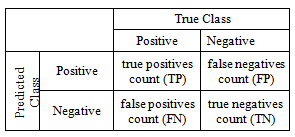
\includegraphics[width=1\textwidth]{figures/im/R2.png}}
		\caption{Confusion Matrix.}
		\label{R2}
		\end{figure}

\item Jelaskan Voting Pada Random Forest Beserta Ilustrasinya \par
Voting pada random forest berguna untuk mengambil nilai pada masing-masing tree yang akan digunakan untuk menentukan hasil final dengan akurasi yang lebih baik. Untuk ilustrasi sederhananya sebagai berikut \ref{R3}
		\begin{figure}[ht]
		\centerline{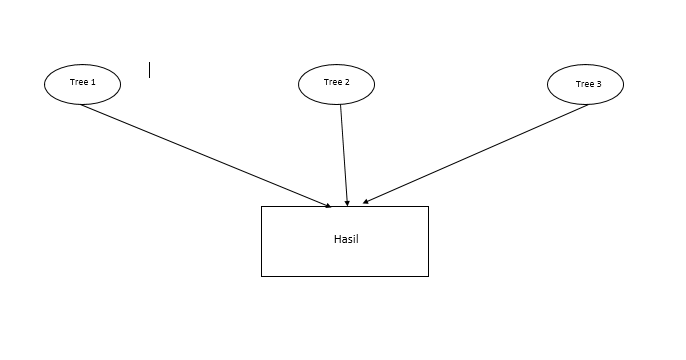
\includegraphics[width=1\textwidth]{figures/im/R3.png}}
		\caption{Voting.}
		\label{R3}
		\end{figure}
\end{enumerate}

\section{Andri Fajar Sunandhar/1164065}
\subsection{Teori}
\begin{enumerate}
\item Apa itu Random Forest Serta Gambar Ilustrasinya \par
Random Forest adalah suatu algoritma yang digunakan pada klasifikasi data dalam jumlah yang besar. Klasifikasi random forest dilakukan melalui penggabungan pohon  dengan melakukan training pada sampel data yang dimiliki. Penggunaan tree yang semakin banyak akan mempengaruhi akurasi yang akan didapatkan menjadi lebih baik. Penentuan klasifikasi dengan random forest diambil berdasarkan hasil voting dari pohon yang terbentuk. Pemenang dari pohon yang terbentuk ditentukan dengan vote terbanyak. Pembangunan pohon  pada random forest sampai dengan mencapai ukuran maksimum dari pohon data. Akan tetapi, pembangunan pohon Random Forest tidak dilakukan pemangkasan  yang merupakan sebuah metode untuk mengurangi kompleksitas ruang. Contoh Ilustrasi sederhana Gambar Random Forest. 
		\begin{figure}[ht]
		\centerline{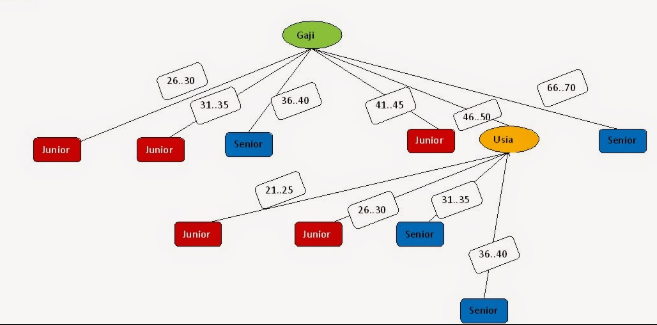
\includegraphics[width=1\textwidth]{figures/AFS/AFS1.png}}
		\caption{Random Forest.}
		\label{AFS1}
		\end{figure}

\item Cara Membaca Dataset
	

		\begin{enumerate}
			\item Buka Anaconda Navigator.
			\item Jalankan Spyder
			\item Import libraries yang dibutuhkan
			\item Masukan kode berikut untuk membaca file Data.csv.
				\begin{figure}[ht]
				\centering
				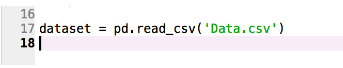
\includegraphics[scale=0.8]{figures/AFS/2.png}
				\caption{Kode membaca file.csv}
				\label{contoh}
				\end{figure}
			\item Jalankan kode tersebut, maka di windiws console akan muncul pesan :
				\begin{figure}[ht]
				\centering
				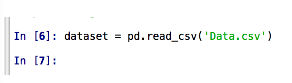
\includegraphics[scale=0.9]{figures/AFS/3.png}
				\caption{ Window Console}
				\label{contoh}
				\end{figure}
			\item Klik variable explorer, maka akan terlihat dataset yang baru ter-import.
				\begin{figure}[ht]
				\centering
				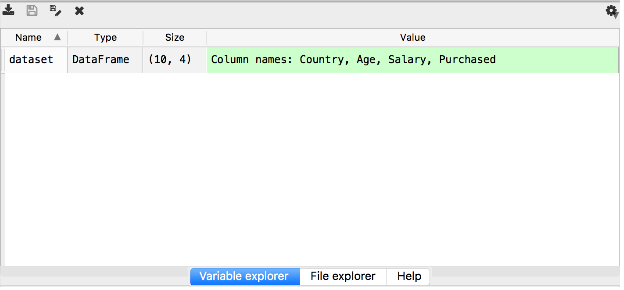
\includegraphics[scale=0.6]{figures/AFS/4.png}
				\caption{Variable Explorer}
				\label{contoh}
				\end{figure}
			\item Kemudian double klik pada dataset cell, maka akan muncul pop-up windows seperti berikut: 
				\begin{figure}[ht]
				\centering
				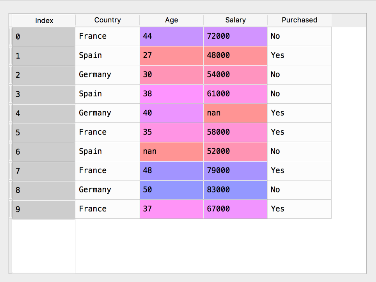
\includegraphics[scale=0.7]{figures/AFS/5.png}
				\caption{ Dataset Cell}
				\label{contoh}
				\end{figure}
			\item Seperti yang terlihat pada gambar tersebut dataset ini memiliki Kolom Country, Age, dan Salary sebagai 		   				independent variable-nya dan kolom Purchased sebagai dependent variable-nya.
			
		\end{enumerate}
	

\item Cross Validation \par
Cross validation adalah metode statistik yang digunakan untuk memperkirakan keterampilan model pembelajaran mesin. Ini biasanya digunakan dalam pembelajaran mesin yang diterapkan untuk membandingkan dan memilih model untuk masalah pemodelan prediktif yang diberikan karena mudah dipahami, mudah diimplementasikan, dan menghasilkan estimasi keterampilan yang umumnya memiliki bias lebih rendah daripada metode lainnya.

\item Arti Score 44\% Pada Random Forest, 27\% Pada Decision Tree dan 29\% Dari SVM \par
\begin{enumerate}
\item Arti Score 44\% \par
Pada Random Forest, Score tersebut merupakan hasil dari akurasi.
\item Arti Score 27\% \par
Pada decission tree adalah presentasi hasil dari perhitungan dataset.
\item Arti Score 29\% Pada SVM \par
merupakan hasil pendekatan jaringan saraf. Jaringan saraf sendiri merupakan komponen jaringan utama dari sistem saraf. Sistem tersebut mengatur dan mengontrol fungsi tubuh dan aktivitas dan terdiri dari dua bagian:  (SSP) yang terdiri dari otak dan sumsum tulang belakang, dan percabangan saraf perifer dari sistem saraf tepi (SST) yang terdapat dalam pengolahan dataset terkait. 
\end{enumerate}

\begin {enumerate}
\item Confusion Matrix Dan Ilustrasinya
\begin{enumerate}
\item Perhitungan confusion matrix adalah sebagai berikut, akan saya beri contoh sederhana yaitu pengambilan keputusan untuk mendapatkan bantuan beasiswa. Saya menggunakan dua atribut, yaitu rekening listrik dan gaji. Ini adalah pohon keputusannya:
 
\begin{figure}[ht]
\centering
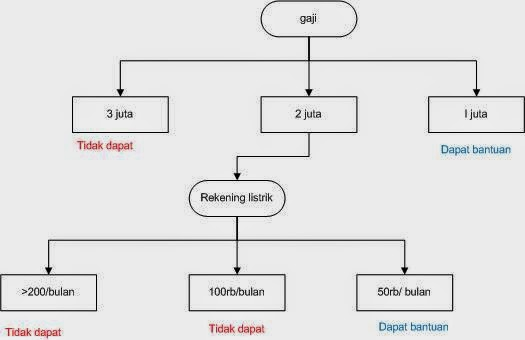
\includegraphics[scale=0.5]{figures/AFS/7.jpg}
\caption{Pohon Keputusan}
\label{contoh}
\end{figure}
\end{enumerate}


Kemudian data testingnya adalah

\begin{figure}[ht]
\centering
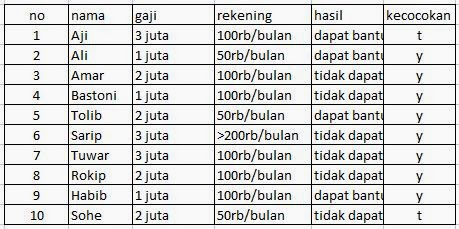
\includegraphics[scale=0.5]{figures/AFS/8.jpg}
\caption{Data Testing}
\label{contoh}
\end{figure}

Yang pertama kita lakukan yaitu mencari 4 nilai yaitu a,b,c, dan d:

 a= 5

 b= 1

 c= 1

 d= 3

Kemudian kita dapat mencari nilai Recall, Precision, accuracy dan Error Rate

 Recall =3/(1+3) = 0,75

 Precision = 3/(1+3) = 0,75

 Accuracy =(5+3)/(5+1+1+3) = 0,8

 Error Rate =(1+1)/(5+1+1+3) = 0,2

\end {enumerate}

\item Jelaskan Voting Pada Random Forest Beserta Ilustrasinya 
\par Voting merupakan metode yang paling umum digunakan dalam random forest. Ketika classifier membuat keputusan, Anda dapat memanfaatkan yang terbaik keputusan umum dan rata-rata yang didefinisikan ke dalam bentuk "voting".
\par Setelah pohon terbentuk,maka akan dilakukan voting pada setiap kelas dari data sampel. Kemudian, mengkombinasikan vote dari setiap kelas kemudian diambil vote yang paling banyak.Dengan menggunakan random forest pada klasifikasi data maka, akan menghasilkan vote yang paling baik. \ref{AFS6}
		\begin{figure}[ht]
		\centerline{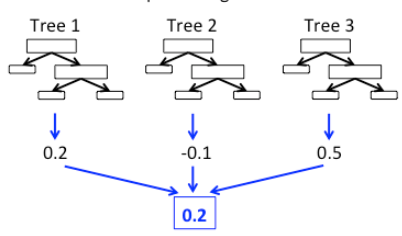
\includegraphics[width=1\textwidth]{figures/AFS/6.png}}
		\caption{Voting.}
		\label{AFS6}
		\end{figure}
\end{enumerate}